\documentclass[12pt]{article}
\usepackage[utf8]{inputenc}

\usepackage{lmodern}

\usepackage{enumitem}
\usepackage[margin=2cm]{geometry}

\usepackage{amsmath, amsfonts, amssymb}
\usepackage{graphicx}
%\usepackage{subfigure}
\usepackage{tikz}
\usepackage{pgfplots}
\usepackage{multicol}

\usepackage{comment}
\usepackage{url}
\usepackage{calc}
\usepackage{subcaption}
\usepackage[indent=0pt]{parskip}
\usepackage{animate}

\usepackage{array}
\usepackage{blkarray,booktabs, bigstrut}
\usepackage{bigints}

\pgfplotsset{compat=1.16}

% MATH commands
\newcommand{\ga}{\left\langle}
\newcommand{\da}{\right\rangle}
\newcommand{\oa}{\left\lbrace}
\newcommand{\fa}{\right\rbrace}
\newcommand{\oc}{\left[}
\newcommand{\fc}{\right]}
\newcommand{\op}{\left(}
\newcommand{\fp}{\right)}

\newcommand{\bi}{\mathbf{i}}
\newcommand{\bj}{\mathbf{j}}
\newcommand{\bk}{\mathbf{k}}
\newcommand{\bF}{\mathbf{F}}

\newcommand{\mR}{\mathbb{R}}

\newcommand{\ra}{\rightarrow}
\newcommand{\Ra}{\Rightarrow}

\newcommand{\sech}{\mathrm{sech}\,}
\newcommand{\csch}{\mathrm{csch}\,}
\newcommand{\curl}{\mathrm{curl}\,}
\newcommand{\dive}{\mathrm{div}\,}

\newcommand{\ve}{\varepsilon}
\newcommand{\spc}{\vspace*{0.5cm}}

\DeclareMathOperator{\Ran}{Ran}
\DeclareMathOperator{\Dom}{Dom}

\newcommand{\exo}[1]{\noindent\textcolor{red}{\fbox{\textbf{Problem {#1}}}\hrulefill}\\\\ }
\newcommand{\qu}[4]{\noindent\textcolor{#4}{\fbox{\textbf{Section {#1} | Problem {#2}}} \hrulefill{{\fbox{\textbf{{#3} Points}}}}\\}}

\newcommand{\semester}{Fall 2023}

\newcommand{\CVup}{%
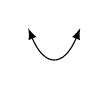
\begin{tikzpicture}
\draw[black, <->, >=latex] (-0.33, 0.5) .. controls (-0.125, 0) and (0.125, 0) .. (0.33, 0.5);
\end{tikzpicture}}

\newcommand{\CVupInc}{%
\begin{tikzpicture}
\draw[black, ->, >=latex] (0,0) .. controls (0.2, 0) and (0.4, 0.2) .. (0.5, 0.5);
\end{tikzpicture}}

\newcommand{\CVupDec}{%
\begin{tikzpicture}[rotate=270]
\draw[black, ->, >=latex] (0,0) .. controls (0.2, 0) and (0.4, 0.2) .. (0.5, 0.5);
\end{tikzpicture}}

\newcommand{\CVdown}{%
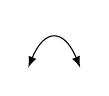
\begin{tikzpicture}
\draw[black, <->, >=latex] (-0.33, -0.5) .. controls (-0.125, 0) and (0.125, 0) .. (0.33, -0.5);
\end{tikzpicture}}

\newcommand{\CVdownInc}{%
\begin{tikzpicture}
\draw[black, ->, >=latex] (-0.5, -0.5) .. controls (-0.5, -0.3) and (-0.5, -0.1) .. (0,0);
\end{tikzpicture}}

\newcommand{\CVdownDec}{%
\begin{tikzpicture}[rotate=-90]
\draw[black, ->, >=latex] (-0.5, -0.5) .. controls (-0.5, -0.3) and (-0.5, -0.1) .. (0,0);
\end{tikzpicture}}

\begin{document}
	\noindent \hrulefill \\
	MATH-244 \semester \hfill Practice Problems Solutions\\
	Section 16.8 \hfill Pierre-Olivier Paris{\'e} \\\vspace*{-1cm}
	
	\noindent\hrulefill
	
	\spc	

	\exo{2}
	By Stokes' Theorem, we have
		\begin{align*}
		\iint_S \curl \vec{F} \, d\vec{S} = \int_C \vec{F} \cdot d \vec{r} .
		\end{align*}
	
	The surface $S$ is the part of the paraboloïd oriented upward. The boundary of $S$ is the circle $x^2 + y^2 = 1$ (when we let $z = 0$ in the equation of the paraboloïd). We parametrize the circle with
		\begin{align*}
		\vec{r} (\theta ) = \left\langle \cos \theta , \sin \theta , 0 \right\rangle \quad (0 \leq \theta \leq 2 \pi ) .
		\end{align*}
	The surface induces the counterclockwise orientation on $C$. Thus, we get
		\begin{align*}
		\iint_S \curl \vec{F} \cdot d \vec{S} &= \int_0^{2\pi} \left\langle \cos^2 \theta \sin (0) , \sin^2 \theta , \cos \theta \sin \theta \right\rangle \cdot \left\langle -\sin \theta , \cos \theta , 0 \right\rangle \, dt \\
		&= \int_0^{2\pi} \sin^2 \theta \cos \theta \, dt = 0 .
		\end{align*}
		
	\spc
	
	\exo{8}
	By Stokes' Theorem, we have
		\begin{align*}
		\int_C \vec{F} \cdot d \vec{r} = \iint_{S} \curl \vec{F} \cdot d \vec{S}
		\end{align*}
	
	The curve $C$ is the boundary of the surface $S$ and a parametrization for the surface $S$ is
		\begin{align*}
		\vec{r} (x, y) = \left\langle x ,y , 1 - 3x - 2y \right\rangle \quad \text{(}0 \leq x \leq 1/3, \, 0 \leq y \leq (1 - 3x)/2 \text{ )} .
		\end{align*}
	Since $C$ is oriented counterclockwise, $S$ must be positively oriented. So, a normal vector to $S$ would be
		\begin{align*}
		\vec{r}_x \times \vec{r}_y = \left\langle 3, 3, 1 \right\rangle .
		\end{align*}
	The $\curl \vec{F}$ is
		\begin{align*}
		\nabla \times \vec{F} = \begin{vmatrix}
		\vec{i} &  \vec{j} & \vec{k} \\
		\partial/\partial x & \partial / \partial y & \partial / \partial z \\
		1 & (x + yz) & xy - \sqrt{z}
		\end{vmatrix}
		= \left\langle x - y , -y , 1 \right\rangle .
		\end{align*}
	So, we obtain
		\begin{align*}
		\curl \vec{F} \cdot (\vec{r}_x \times \vec{r}_y ) = 3x - 3y - 3y + 1 = 3x - 6y + 1 .
		\end{align*}
	Thus, we finally obtain
		\begin{align*}
		\int_C \vec{F} \cdot d\vec{r} = \int_0^{1/3} \int_0^{(1 - 3x)/2} 3x - 6y + 1 \, dy dx = 1/36 .
		\end{align*}

\end{document}